\documentclass{article}

\usepackage{microtype}
\usepackage{graphicx}
\usepackage{subfigure}
\usepackage{booktabs}

\usepackage{fontawesome}
\usepackage{hyperref}
\usepackage{url}

% Attempt to make hyperref and algorithmic work together better:
\newcommand{\theHalgorithm}{\arabic{algorithm}}

\usepackage[accepted]{icml2020}

\icmltitlerunning{Guideline and Formatting Instructions for Final Projects (Machine Learning 2023 Course)}

\begin{document}

\twocolumn[
  \icmltitle{Guideline and Formatting Instructions for Final Projects\\(Machine Learning 2023 Course)}

  \icmlsetsymbol{equal}{*}

  \begin{icmlauthorlist}
    \icmlauthor{Alexander Korotin}{sk}
    \icmlauthor{Evgeny Burnaev}{sk}
    % \icmlauthor{Example}{equal,other}
  \end{icmlauthorlist}

  \icmlaffiliation{sk}{Skolkovo Institute of Science and Technology, Moscow, Russia}
  % \icmlaffiliation{other}{Other affiliation}

  \icmlcorrespondingauthor{Alexander Korotin}{a.korotin@skoltech.ru}

  \icmlkeywords{Final Project, Machine Learning, Skoltech}

  \vskip 0.3in
]
\printAffiliationsAndNotice{}  % leave blank if no need to mention equal contribution
% \printAffiliationsAndNotice{\icmlEqualContribution} % otherwise use the standard text.
\begin{abstract}
  This document provides guidelines and a basic template for the final project reports at \textbf{Machine Learning 2023 course} organized by \textit{Skolkovo University of Science and Technology} (\href{skoltech.ru}{Skoltech}). The document is based on \href{https://icml.cc/Conferences/2020/Dates}{ICML 2020} submission guidelines. An abstract must be a single paragraph, ideally between 4--6 sentences long.
\end{abstract}

\underline{\textbf{Github repo:}} \href{github.com}{your project github repo link here}\newline
\underline{\textbf{Presentation file:}} \href{github.com}{your link here to presentation file in github }

\section{Online Submission}
\label{submission}

Submission of final project reports is performed entirely online, via \href{github.com}{Github project repo}. The guidelines below are enforced for all submissions. Here is a brief summary:
\begin{itemize}
  \item Students have to submit into Github repo two *.pdf files: \textbf{presentation} and \textbf{report}.
  \item The source of this guideline, based on the icml format, should be used as the \LaTeX project \textbf{report} template for all projects. Do not alter the style template; in particular, do not increase the report size by adding extra vertical spaces.
  \item Submitted projects must be from \textbf{four} (full) to \textbf{seven} pages long, \textbf{not including references and appendices}. Projects which do not obey this rule will automatically be rejected and receive zero grade.
  \item Students must \textbf{include author information} in reports.
  \item Your report should be in \textbf{10 point Times font}.
  \item Place figure captions \emph{under} the figure (and omit titles from inside
    the graphic file itself). Place table captions \emph{over} the table.
  \item Keep your abstract brief and self-contained, one paragraph and roughly
    4--6 sentences describing the motivation and key results of your project.
\end{itemize}

\subsection{Submitting Project Reports}

\textbf{Project Report Submission Deadline:} The deadline for project report submission that is announced on the course canvas page is strict. If your full submission does not reach us on time, it will not be
considered for grading.

Students must provide their manuscripts in \textbf{PDF} format.
% Additionally, students have to submit complete \LaTeX\@ source packed in a \texttt{*.zip} format.

The usage of \textbf{Word} is prohibited. Really. We're not joking. Don't send Word or PDFs compiled from Word.

\textbf{Graphics files} should be of a reasonable size, and included from
an appropriate format. Use vector formats (.eps/.pdf) for plots,
lossless bitmap formats (.png) for raster graphics with sharp lines, and
jpeg for photo-like images.

\section{Content of the Project Report}
The project report should be a solid logical high quality text describing your project and obtained results. The quality of the report should equal to a publication that can go into a minor venue. \textbf{The sectioning should be as follows:}

\underline{\textbf{Abstract.}} Brief and self-contained text. One paragraph (roughly 4--6 sentences) describing the motivation and key results of your project.

Between abstract and Introduction you must insert the links to your \textbf{github repo} and \textbf{ presentation} of the project.

\underline{\textbf{Introduction.}} A gentle introduction to the topic of your report, deeper explanation of motivation (mentioning some recent related work on your topic). The introduction must end with the phrase \textbf{the main contributions of this report are as follows} and following concise but still very clear list of 2-4 tasks, problems, improvements, replications, experiments (listed as bullet points) that you performed in your project. This is a usual practice to make the contributions explicit to readers and reviewers. For example, see \cite{arjovsky2017wasserstein,NIPS20198433} or almost any other conference paper.

\underline{\textbf{Preliminaries}} (optional). In some cases, it is reasonable to devote a specific section for notation, key concepts, definitions (especially if the topic is not widespread around data science and machine learning community). Students may include the contents of this section to introduction or related work section, depending on the situation.

\underline{\textbf{Related work}} Review of old, recent and state-of-the art methods for solving the problem students encounter in their project. At least 4-5 references should be mentioned with a brief discussion of their drawbacks and advantages.

\underline{\textbf{Algorithms and Models}} and \underline{\textbf{Experiments and Results.}}

Two main sections describing key students' results. All the relevant content should be distributed among these sections based on the topic of project, stated goals, project plan and students' decision. In general, these sections should contain clear experimental setup and a  link to a \textbf{github repo} (again!) with a fully reproducible code. \textbf{Projects without a github repo with a reproducible code will be graded as zero.}

Students have to explicitly describe the algorithms, models, methods, approaches they used for solving their project's problem. Students should explain the motivation for choosing the models, possible benefits and drawbacks of the choice in application to their problem. The used metrics for accessing the quality of the results should also be described.

The section(s) must contain a \textbf{complete description of the datasets} used for experiments with all the required download links. This includes number of features, samples, types of features (categorial, real, pixels, etc.), description of key features, etc. If well-known datasets are used, e.g. MNIST, CIFAR, etc., it is enough to put a link to a dataset (or related paper) without a detailed description.

All the \textbf{preprocessing} and data-handling steps should be presented in these sections. Make sure to answer relevant questions, e.g. the following ones: How data was normalized? How data augmentation was done? How data was cleaned from outliers or anomalies? How the data was splitted for train, test, validation?

All \textbf{training parameters} should be listed. Which methods did you try and with which parameters (e.g. neural network architectures, weight initialization, optimizers, optimizer parameters, number of epochs, iterations, cross validation, exact number of restarts, etc.)?

We highly encourage students to additionally present experimental results in a form of \textbf{tables and plots} (e.g. generated images for projects related to image generation, segmented images for project related to segmentation, table with scores for projects related to prediction, etc.). All the experimental results must be properly discussed and explained. If you experience problems with creating tables in \LaTeX, use e.g. \href{https://www.tablesgenerator.com}{this online tool} or any its analog. In Python's \textit{Pandas} library there are also methods to convert \href{https://pandas.pydata.org/pandas-docs/stable/reference/api/pandas.DataFrame.to_latex.html}{\textbf{pd.DataFrame}} to \LaTeX  .

\underline{\textbf{Conclusion}} Concise description of experimental results and outcomes, including possible directions for further work.

\underline{\textbf{References.}} For references, we highly encourage students to use \texttt{references.bib} file provided with the template. To add a reference to the \texttt{.bib}, use its Bib-Tex, e.g.  provided by \href{scholar.google.com}{Google Scholar}. To cite a reference, use \texttt{\textbackslash cite\{\}}. Students are expected to refer at least to $5$ relevant papers.

\underline{\textbf{Appendix \ref{appendix-contrib}: Contributions of the Team Members}}.

In this \textbf{mandatory} appendix, the contribution of each team member to the project has to be clarified.

\underline{\textbf{Appendix \ref{appendix-checklist}: Reproducibility Checklist}} Students \textbf{must} answer all the questions listed in the Appendix \ref{appendix-checklist} (end of this document) regarding reproducibility of the project results.

Filling appendices \ref{appendix-contrib} and  \ref{appendix-checklist} is mandatory. \textbf{Projects with empty or incomplete appendices will be graded as zero.}

\section{Format of the Project Report}

The source of this guideline, based on the icml format, should be used as the \LaTeX project report template for all projects.

\subsection{Dimensions}

The text of the report should be formatted in two columns, with an
overall width of 6.75~inches, height of 9.0~inches, and 0.25~inches
between the columns. The left margin should be 0.75~inches and the top
margin 1.0~inch (2.54~cm). The right and bottom margins will depend on
whether you print on US letter or A4 paper.

The paper body should be set in 10~point type with a vertical spacing
of 11~points.

\subsection{Title}

The project title should be set in 14~point bold type and centered
between two horizontal rules that are 1~point thick, with 1.0~inch
between the top rule and the top edge of the page. Capitalize the
first letter of content words and put the rest of the title in lower
case.

\subsection{Abstract}

The paper abstract should begin in the left column, 0.4~inches below the final
address. The heading `Abstract' should be centered, bold, and in 11~point type.
The abstract body should use 10~point type, with a vertical spacing of
11~points, and should be indented 0.25~inches more than normal on left-hand and
right-hand margins. Insert 0.4~inches of blank space after the body. Keep your
abstract brief and self-contained, limiting it to one paragraph and roughly 4--6
sentences.

\subsection{Partitioning the Text}

You should organize your report into sections and paragraphs to help
readers place a structure on the material and understand its
contributions.

\subsubsection{Sections and Subsections}

Section headings should be numbered, flush left, and set in 11~pt bold
type with the content words capitalized. Leave 0.25~inches of space
before the heading and 0.15~inches after the heading.

Similarly, subsection headings should be numbered, flush left, and set
in 10~pt bold type with the content words capitalized. Leave
0.2~inches of space before the heading and 0.13~inches afterward.

Finally, subsubsection headings should be numbered, flush left, and
set in 10~pt small caps with the content words capitalized. Leave
0.18~inches of space before the heading and 0.1~inches after the
heading.

Please use no more than three levels of headings.

\subsubsection{Paragraphs and Footnotes}

Within each section or subsection, you should further partition the
paper into paragraphs. Do not indent the first line of a given
paragraph, but insert a blank line between succeeding ones.

You can use footnotes\footnote{Footnotes
should be complete sentences.} to provide readers with additional
information about a topic without interrupting the flow of the paper.
Indicate footnotes with a number in the text where the point is most
relevant. Place the footnote in 9~point type at the bottom of the
column in which it appears. Precede the first footnote in a column
with a horizontal rule of 0.8~inches.\footnote{Multiple footnotes can
  appear in each column, in the same order as they appear in the text,
but spread them across columns and pages if possible.}

\begin{figure}[ht]
  \vskip 0.2in
  \begin{center}
    \centerline{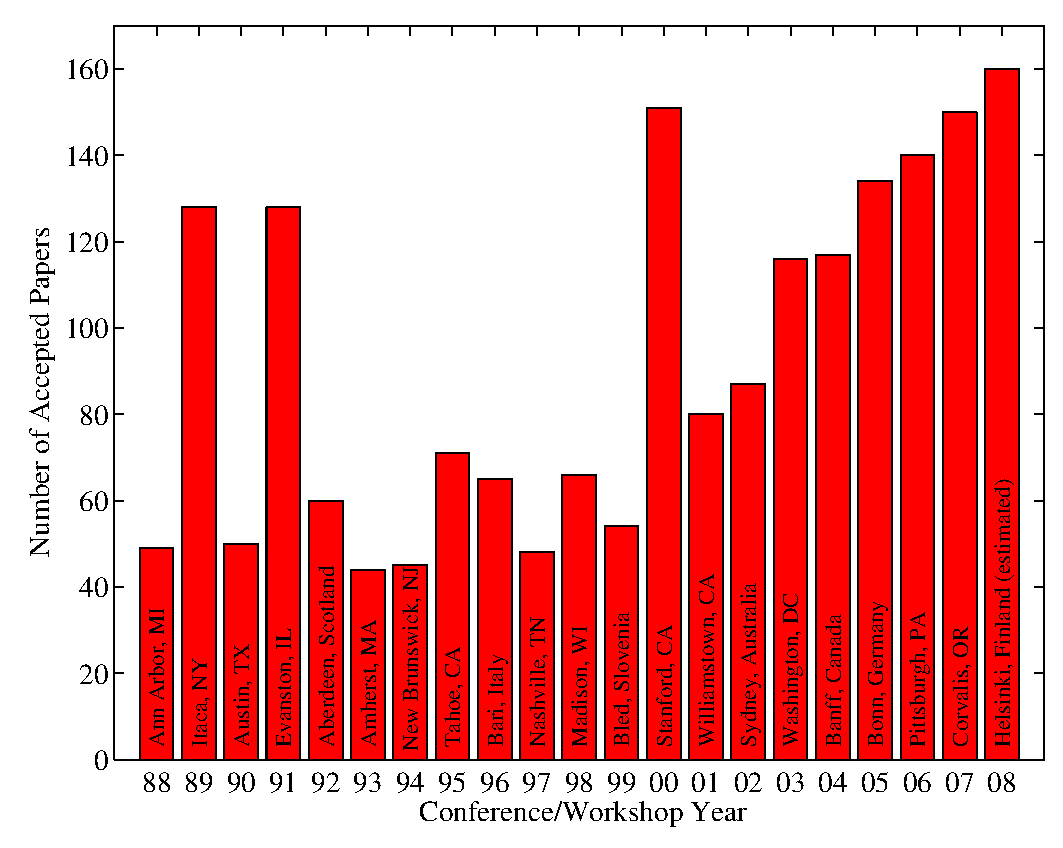
\includegraphics[width=\columnwidth]{icml_numpapers}}
    \caption{Historical locations and number of accepted papers for International
      Machine Learning Conferences (ICML 1993 -- ICML 2008) and International
      Workshops on Machine Learning (ML 1988 -- ML 1992). At the time this figure was
      produced, the number of accepted papers for ICML 2008 was unknown and instead
    estimated.}
    \label{icml-historical}
  \end{center}
  \vskip -0.2in
\end{figure}

\subsection{Figures}

You may want to include figures in the paper to illustrate
your approach and results. Such artwork should be centered,
legible, and separated from the text. Lines should be dark and at
least 0.5~points thick for purposes of reproduction, and text should
not appear on a gray background.

Label all distinct components of each figure. If the figure takes the
form of a graph, then give a name for each axis and include a legend
that briefly describes each curve. Do not include a title inside the
figure; instead, the caption should serve this function.

Number figures sequentially, placing the figure number and caption
\emph{after} the graphics, with at least 0.1~inches of space before
the caption and 0.1~inches after it, as in
Figure~\ref{icml-historical}. The figure caption should be set in
9~point type and centered unless it runs two or more lines, in which
case it should be flush left. You may float figures to the top or
bottom of a column, and you may set wide figures across both columns
(use the environment \texttt{figure*} in \LaTeX). Always place
two-column figures at the top or bottom of the page.

\subsection{Algorithms}

Please use the ``algorithm'' and ``algorithmic''
environments to format pseudocode. These require
the corresponding stylefiles, algorithm.sty and
algorithmic.sty, which are supplied with this package.
Algorithm~\ref{alg:example} shows an example.

\begin{algorithm}[tb]
  \caption{Bubble Sort}
  \label{alg:example}
  \begin{algorithmic}
    \STATE {\bfseries Input:} data $x_i$, size $m$
    \REPEAT
    \STATE Initialize $noChange = true$.
    \FOR{$i=1$ {\bfseries to} $m-1$}
    \IF{$x_i > x_{i+1}$}
    \STATE Swap $x_i$ and $x_{i+1}$
    \STATE $noChange = false$
    \ENDIF
    \ENDFOR
    \UNTIL{$noChange$ is $true$}
  \end{algorithmic}
\end{algorithm}

\subsection{Tables}

You may also want to include tables that summarize material. Like
figures, these should be centered, legible, and numbered consecutively.
However, place the title \emph{above} the table with at least
0.1~inches of space before the title and the same after it, as in
Table~\ref{sample-table}. The table title should be set in 9~point
type and centered unless it runs two or more lines, in which case it
should be flush left.

% Note use of \abovespace and \belowspace to get reasonable spacing
% above and below tabular lines.

\begin{table}[t]
  \caption{Classification accuracies for naive Bayes and flexible
  Bayes on various data sets.}
  \label{sample-table}
  \vskip 0.15in
  \begin{center}
    \begin{small}
      \begin{sc}
        \begin{tabular}{lcccr}
          \toprule
          Data set & Naive & Flexible & Better? \\
          \midrule
          Breast    & 95.9$\pm$ 0.2& 96.7$\pm$ 0.2& $\surd$ \\
          Cleveland & 83.3$\pm$ 0.6& 80.0$\pm$ 0.6& $\times$\\
          Glass2    & 61.9$\pm$ 1.4& 83.8$\pm$ 0.7& $\surd$ \\
          Credit    & 74.8$\pm$ 0.5& 78.3$\pm$ 0.6&         \\
          Horse     & 73.3$\pm$ 0.9& 69.7$\pm$ 1.0& $\times$\\
          Meta      & 67.1$\pm$ 0.6& 76.5$\pm$ 0.5& $\surd$ \\
          Pima      & 75.1$\pm$ 0.6& 73.9$\pm$ 0.5&         \\
          Vehicle   & 44.9$\pm$ 0.6& 61.5$\pm$ 0.4& $\surd$ \\
          \bottomrule
        \end{tabular}
      \end{sc}
    \end{small}
  \end{center}
  \vskip -0.1in
\end{table}

Tables contain textual material, whereas figures contain graphical material.
Specify the contents of each row and column in the table's topmost
row. Again, you may float tables to a column's top or bottom, and set
wide tables across both columns. Place two-column tables at the
top or bottom of the page.

\subsection{Citations and References}

Please use APA reference format regardless of your formatter
or word processor. If you rely on the \LaTeX\/ bibliographic
facility, use \texttt{natbib.sty} and \texttt{icml2020.bst}
included in the style-file package to obtain this format.

Citations within the text should include the authors' last names and
year. If the authors' names are included in the sentence, place only
the year in parentheses, for example when referencing Arthur Samuel's
pioneering work \yrcite{Samuel59}. Otherwise place the entire
reference in parentheses with the authors and year separated by a
comma \cite{Samuel59}. List multiple references separated by
semicolons \cite{kearns89,Samuel59,mitchell80}. Use the `et~al.'
construct only for citations with three or more authors or after
listing all authors to a publication in an earlier reference \cite{MachineLearningI}.

Use an unnumbered first-level section heading for the references, and use a
hanging indent style, with the first line of the reference flush against the
left margin and subsequent lines indented by 10 points. The references at the
end of this document give examples for journal articles \cite{Samuel59},
conference publications \cite{langley00}, book chapters \cite{Newell81}, books
\cite{DudaHart2nd}, edited volumes \cite{MachineLearningI}, technical reports
\cite{mitchell80}, and dissertations \cite{kearns89}.

Please put some effort into making references complete, presentable, and
consistent. If using bibtex, please protect capital letters of names and
abbreviations in titles, for example, use \{B\}ayesian or \{L\}ipschitz
in your .bib file.

\bibliography{references}
\bibliographystyle{icml2020}

%%%%%%%%%%%%%%%%%%%%%%%%%%%%%%%%%%%%%%%%%%%%%%%%%%%%%%%%%%%%%%%%%%%%%%%%%%%%%%%
%%%%%%%%%%%%%%%%%%%%%%%%%%%%%%%%%%%%%%%%%%%%%%%%%%%%%%%%%%%%%%%%%%%%%%%%%%%%%%%
% DELETE THIS PART. DO NOT PLACE CONTENT AFTER THE REFERENCES!
%%%%%%%%%%%%%%%%%%%%%%%%%%%%%%%%%%%%%%%%%%%%%%%%%%%%%%%%%%%%%%%%%%%%%%%%%%%%%%%
%%%%%%%%%%%%%%%%%%%%%%%%%%%%%%%%%%%%%%%%%%%%%%%%%%%%%%%%%%%%%%%%%%%%%%%%%%%%%%%

\newpage
\appendix
\section{Team member's contributions}
\label{appendix-contrib}
Explicitly stated contributions of each team member to the final project.
\subsection*{Name 1 (20\% of work)}
\begin{itemize}
  \item Reviewing literate on the topic (3 papers)
  \item Coding the main algorithm
  \item Experimenting with model parameters on MNIST dataset
  \item Preparing the GitHub Repo
  \item Preparing the Section N of this report
  \item ...
\end{itemize}

\subsection*{Name 2 (25\% of work)}
\begin{itemize}
  \item ...
\end{itemize}

\subsection*{Name 3 (55\% of work)}
\begin{itemize}
  \item ...
\end{itemize}

\clearpage
\section{Reproducibility checklist}
\label{appendix-checklist}
Answer the questions of following reproducibility checklist. If necessary, you may leave a comment.
\begin{enumerate}
  \item A ready code was used in this project, e.g. for replication project the code from the corresponding paper was used.
    \begin{itemize}
      \item [\faCheckSquareO] Yes.
      \item [\faSquareO] No.
      \item [\faSquareO] Not applicable.
    \end{itemize}

    \textbf{General comment:} If the answer is \textbf{yes}, students must \underline{explicitly clarify} to which extent (e.g. which percentage of your code did you write on your own?) and which code was used.

    \textbf{Students' comment:} None
  \item A clear description of the mathematical setting, algorithm, and/or model is included in the report.
    \begin{itemize}
      \item [\faSquareO] Yes.
      \item [\faSquareO] No.
      \item [\faSquareO] Not applicable.
    \end{itemize}

    \textbf{Students' comment:} None

  \item A link to a downloadable source code, with specification of all dependencies, including external libraries is included in the report.
    \begin{itemize}
      \item [\faSquareO] Yes.
      \item [\faSquareO] No.
      \item [\faSquareO] Not applicable.
    \end{itemize}

    \textbf{Students' comment:} None

  \item A complete description of the data collection process, including sample size, is included in the report.
    \begin{itemize}
      \item [\faSquareO] Yes.
      \item [\faSquareO] No.
      \item [\faSquareO] Not applicable.
    \end{itemize}

    \textbf{Students' comment:} None

  \item A link to a downloadable version of the dataset or simulation environment is included in the report.
    \begin{itemize}
      \item [\faSquareO] Yes.
      \item [\faSquareO] No.
      \item [\faSquareO] Not applicable.
    \end{itemize}

    \textbf{Students' comment:} None

  \item An explanation of any data that were excluded, description of any pre-processing step are included in the report.
    \begin{itemize}
      \item [\faSquareO] Yes.
      \item [\faSquareO] No.
      \item [\faSquareO] Not applicable.
    \end{itemize}

    \textbf{Students' comment:} None

  \item An explanation of how samples were allocated for training, validation and testing is included in the report.
    \begin{itemize}
      \item [\faSquareO] Yes.
      \item [\faSquareO] No.
      \item [\faSquareO] Not applicable.
    \end{itemize}

    \textbf{Students' comment:} None

  \item The range of hyper-parameters considered, method to select the best hyper-parameter
    configuration, and specification of all hyper-parameters used to generate results are included in the report.
    \begin{itemize}
      \item [\faSquareO] Yes.
      \item [\faSquareO] No.
      \item [\faSquareO] Not applicable.
    \end{itemize}

    \textbf{Students' comment:} None

  \item The exact number of evaluation runs is included.
    \begin{itemize}
      \item [\faSquareO] Yes.
      \item [\faSquareO] No.
      \item [\faSquareO] Not applicable.
    \end{itemize}

    \textbf{Students' comment:} None

  \item A description of how experiments have been conducted is included.
    \begin{itemize}
      \item [\faSquareO] Yes.
      \item [\faSquareO] No.
      \item [\faSquareO] Not applicable.
    \end{itemize}

    \textbf{Students' comment:} None

  \item A clear definition of the specific measure or statistics used to report results is included in the report.
    \begin{itemize}
      \item [\faSquareO] Yes.
      \item [\faSquareO] No.
      \item [\faSquareO] Not applicable.
    \end{itemize}

    \textbf{Students' comment:} None

  \item Clearly defined error bars are included in the report.
    \begin{itemize}
      \item [\faSquareO] Yes.
      \item [\faSquareO] No.
      \item [\faSquareO] Not applicable.
    \end{itemize}

    \textbf{Students' comment:} None

  \item A description of the computing infrastructure used is included in the report.
    \begin{itemize}
      \item [\faSquareO] Yes.
      \item [\faSquareO] No.
      \item [\faSquareO] Not applicable.
    \end{itemize}

    \textbf{Students' comment:} None
\end{enumerate}

\end{document}

% This document was modified from the file originally made available by
% Pat Langley and Andrea Danyluk for ICML-2K. This version was created
% by Iain Murray in 2018, and modified by Alexandre Bouchard in
% 2019 and 2020. Previous contributors include Dan Roy, Lise Getoor and Tobias
% Scheffer, which was slightly modified from the 2010 version by
% Thorsten Joachims & Johannes Fuernkranz, slightly modified from the
% 2009 version by Kiri Wagstaff and Sam Roweis's 2008 version, which is
% slightly modified from Prasad Tadepalli's 2007 version which is a
% lightly changed version of the previous year's version by Andrew
% Moore, which was in turn edited from those of Kristian Kersting and
% Codrina Lauth. Alex Smola contributed to the algorithmic style files.
